\begin{question}
\noindent A historian is studying an old star-chart in which a triangular constellation marker $T$, with vertices $A(2,1)$, $B(2,3)$ and $C(5,1)$, is reflected in the mirror line $y = x$ to produce an image marker $T'$.

\begin{center}
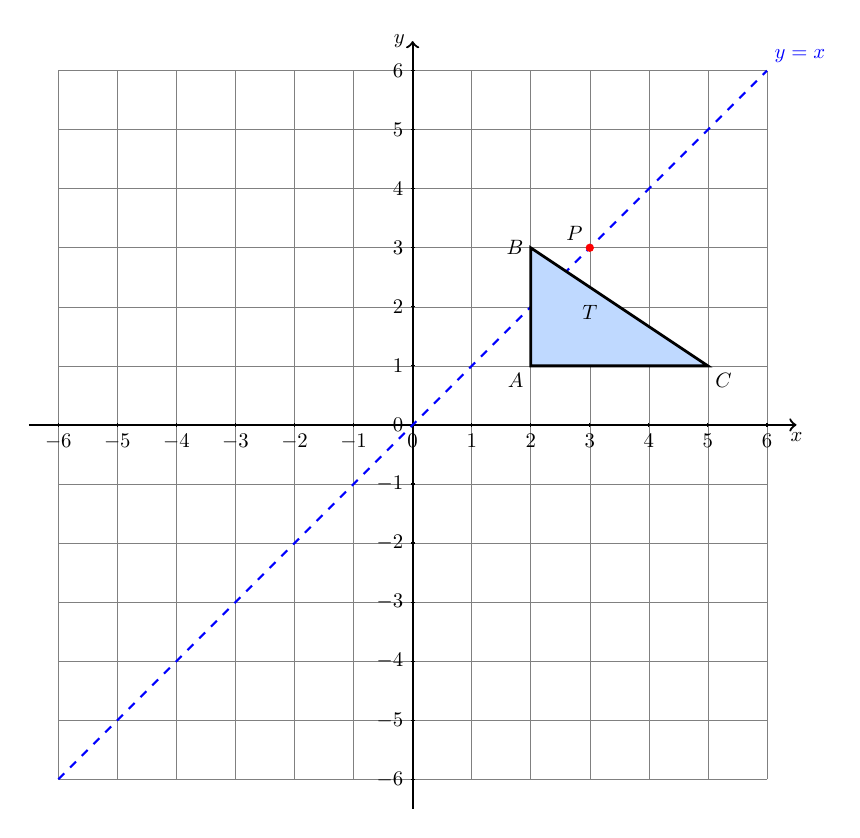
\begin{tikzpicture}[scale=0.75, transform shape]
    \def\axisLimit{6}

    \definecolor{borderColour}{HTML}{000000}
    \definecolor{fillColourT}{HTML}{BFD9FF}
    \definecolor{fillColourTp}{HTML}{FFD8B0}

    % Draw grid
    \draw[step=1cm,gray,very thin] (-\axisLimit,-\axisLimit) grid (\axisLimit,\axisLimit);

    % Draw axes
    \draw[thick,->] (-\axisLimit-0.5,0) -- (\axisLimit+0.5,0) node[anchor=north] {$x$};
    \draw[thick,->] (0,-\axisLimit-0.5) -- (0,\axisLimit+0.5) node[anchor=east] {$y$};

    % Label x-axis and y-axis
    \foreach \x in {-\axisLimit,...,\axisLimit}
        \draw (\x cm,1pt) -- (\x cm,-1pt) node[anchor=north] {$\x$};
    \foreach \y in {-\axisLimit,...,\axisLimit}
        \draw (1pt,\y cm) -- (-1pt,\y cm) node[anchor=east] {$\y$};

    % Mirror line y = x
    \draw[thick, dashed, blue] (-\axisLimit,-\axisLimit) -- (\axisLimit,\axisLimit) node[above right]{$y=x$};

    % Triangle T: A(2,1), B(2,3), C(5,1)
    \coordinate (A) at (2,1);
    \coordinate (B) at (2,3);
    \coordinate (C) at (5,1);
    \filldraw[fill=fillColourT, draw=borderColour, line width=1pt] (A) -- (B) -- (C) -- cycle;
    \node[below left] at (A) {$A$};
    \node[left] at (B) {$B$};
    \node[below right] at (C) {$C$};
    \node at (3,1.9) {$T$};

    % Point P(3,3) marked on the mirror line
    \coordinate (P) at (3,3);
    \fill[red] (P) circle (2pt);
    \node[above left] at (P) {$P$};

\end{tikzpicture}
\end{center}

\noindent The point $P$ has coordinates $(3, 3)$ and lies on the mirror line $y = x$, as shown on the diagram.

\noindent Show that $P$ is an invariant point under this reflection, i.e.\ show that $P$ maps to itself.

\vspace{4cm}

\answermarks{3}
\end{question}
